\documentclass[11pt,letterpaper]{article}

% ── Packages ──────────────────────────────────────────────────
\usepackage[margin=1in]{geometry}
\usepackage{tikz}
\usetikzlibrary{
  arrows.meta,
  positioning,
  shapes.geometric,
  backgrounds,
  fit,
  calc,
  decorations.pathmorphing,
  patterns
}
\usepackage{booktabs}
\usepackage{xcolor}
\usepackage{enumitem}
\usepackage{amsmath,amssymb}
\usepackage{microtype}
\usepackage{hyperref}
\usepackage{caption}
\usepackage{subcaption}
\usepackage{fancyhdr}
\usepackage[T1]{fontenc}
\usepackage{lmodern}

% ── Colors ────────────────────────────────────────────────────
\definecolor{eqgreen}{HTML}{2E7D32}
\definecolor{eqlight}{HTML}{E8F5E9}
\definecolor{csred}{HTML}{C62828}
\definecolor{cslight}{HTML}{FFEBEE}
\definecolor{warnambr}{HTML}{F57F17}
\definecolor{warnlight}{HTML}{FFF8E1}
\definecolor{graphblue}{HTML}{1565C0}
\definecolor{graphlight}{HTML}{E3F2FD}
\definecolor{codegray}{HTML}{37474F}
\definecolor{codelightgray}{HTML}{ECEFF1}
\definecolor{inventedpurp}{HTML}{6A1B9A}
\definecolor{inventedlight}{HTML}{F3E5F5}

% ── Page style ────────────────────────────────────────────────
\pagestyle{fancy}
\fancyhf{}
\rhead{\footnotesize Atlas Graph Audit}
\lhead{\footnotesize NestedLearning / HADES}
\cfoot{\thepage}

% ── Title ─────────────────────────────────────────────────────
\title{%
  \textbf{Atlas-MAG Graph Audit}\\[0.3em]
  \large Correct Math, Wrong Ontology:\\
  How the Graph Catches What Testing Cannot%
}
\author{%
  NestedLearning Project\\
  \texttt{HADES\_DATABASE=NL}%
}
\date{February 2026}

\begin{document}
\maketitle
\thispagestyle{fancy}

% ══════════════════════════════════════════════════════════════
\section{Executive Summary}
% ══════════════════════════════════════════════════════════════

The Atlas-MAG\_OmegaRule implementation (4 months, 4{,}805 lines, 109 tests,
85.9\% NIAH accuracy) was built \emph{without} the NL graph methodology.
Post-hoc audit against the HADES graph reveals a consistent pattern:

\begin{center}
\fbox{\parbox{0.85\textwidth}{%
  \textbf{The mathematical layer is correct.}
  Every equation---Omega loss (Eq~9), momentum (Eq~32),
  NS-5 update (Eq~33), polynomial features (Eqs~4--5),
  MAG gating---is faithfully implemented.\\[0.5em]
  \textbf{The architectural layer is wrong.}
  The code introduces structural concepts (separate memory modules,
  training/inference mode distinction, multiple external APIs, invented
  persistent memory) that do not exist in the paper's ontology.\\[0.5em]
  \textbf{All 109 tests pass.} Tests verify math. The graph verifies ontology.
  These are orthogonal.
}}
\end{center}

This report documents the specific structural breaks with graph diagrams
suitable for inclusion in the methodology article.

% ══════════════════════════════════════════════════════════════
\section{Figure 1: The Two-Layer Audit}
% ══════════════════════════════════════════════════════════════

The graph enforces compliance at two layers: \textbf{equations} (mathematical
correctness) and \textbf{code smells} (structural correctness). The old
implementation passes the first and fails the second.

\begin{figure}[h!]
\centering
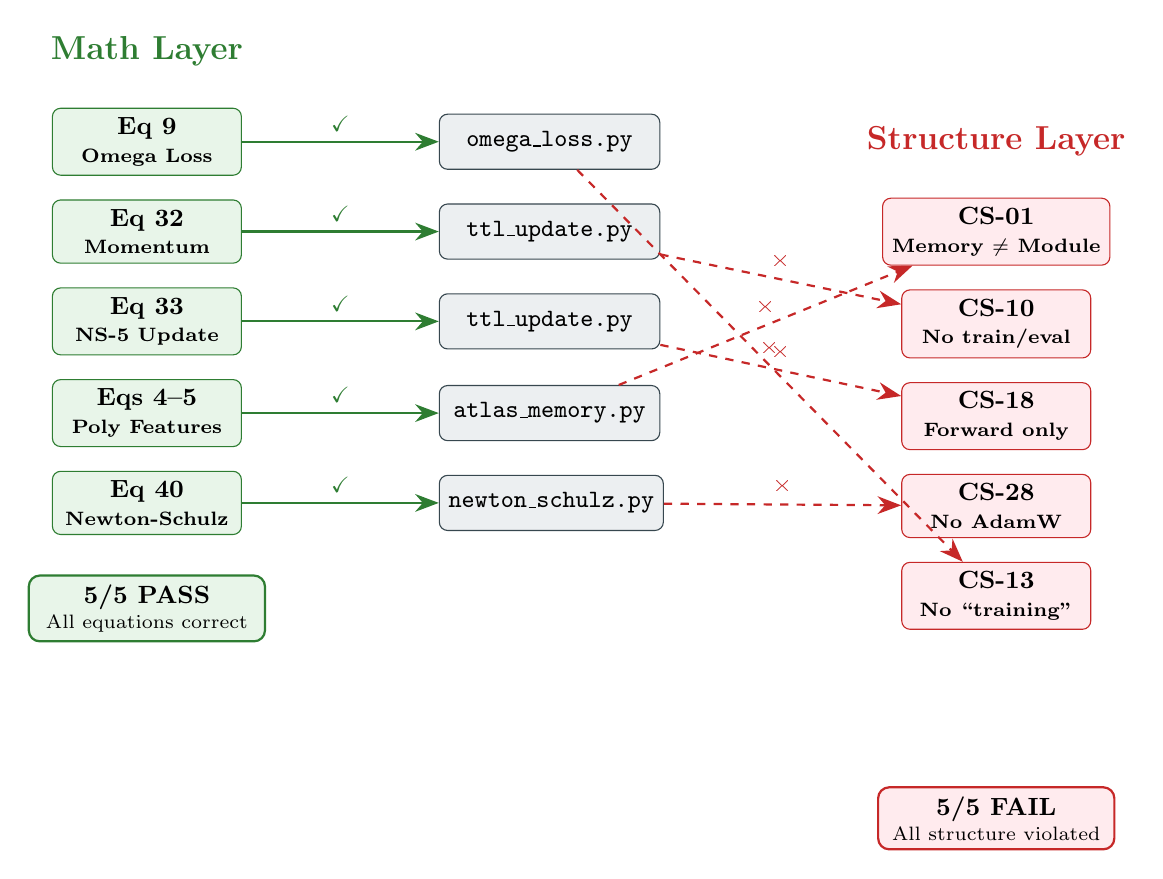
\begin{tikzpicture}[
  node distance=0.6cm and 1.0cm,
  every node/.style={font=\small},
  eqnode/.style={
    rectangle, rounded corners=3pt, draw=eqgreen, fill=eqlight,
    minimum width=2.4cm, minimum height=0.7cm, align=center,
    font=\small\bfseries
  },
  csnode/.style={
    rectangle, rounded corners=3pt, draw=csred, fill=cslight,
    minimum width=2.4cm, minimum height=0.7cm, align=center,
    font=\small\bfseries
  },
  codenode/.style={
    rectangle, rounded corners=3pt, draw=codegray, fill=codelightgray,
    minimum width=2.8cm, minimum height=0.7cm, align=center,
    font=\small\ttfamily
  },
  passarrow/.style={-{Stealth[length=3mm]}, thick, eqgreen},
  failarrow/.style={-{Stealth[length=3mm]}, thick, csred, dashed},
  label/.style={font=\footnotesize, midway}
]

% ── Column 1: Equations (Math Layer) ──
\node[font=\bfseries\large, eqgreen] (mathtitle) at (0,0) {Math Layer};
\node[eqnode, below=0.4cm of mathtitle] (eq9) {Eq 9\\[-1pt]\scriptsize Omega Loss};
\node[eqnode, below=0.3cm of eq9] (eq32) {Eq 32\\[-1pt]\scriptsize Momentum};
\node[eqnode, below=0.3cm of eq32] (eq33) {Eq 33\\[-1pt]\scriptsize NS-5 Update};
\node[eqnode, below=0.3cm of eq33] (eq45) {Eqs 4--5\\[-1pt]\scriptsize Poly Features};
\node[eqnode, below=0.3cm of eq45] (eq40) {Eq 40\\[-1pt]\scriptsize Newton-Schulz};

% ── Column 2: Code Modules ──
\node[codenode, right=2.5cm of eq9] (omegaloss) {omega\_loss.py};
\node[codenode, right=2.5cm of eq32] (ttlstep) {ttl\_update.py};
\node[codenode, right=2.5cm of eq33] (ttlns) {ttl\_update.py};
\node[codenode, right=2.5cm of eq45] (polyfeat) {atlas\_memory.py};
\node[codenode, right=2.5cm of eq40] (ns5) {newton\_schulz.py};

% ── Green arrows (math traces) ──
\draw[passarrow] (eq9) -- node[above, label, eqgreen] {\checkmark} (omegaloss);
\draw[passarrow] (eq32) -- node[above, label, eqgreen] {\checkmark} (ttlstep);
\draw[passarrow] (eq33) -- node[above, label, eqgreen] {\checkmark} (ttlns);
\draw[passarrow] (eq45) -- node[above, label, eqgreen] {\checkmark} (polyfeat);
\draw[passarrow] (eq40) -- node[above, label, eqgreen] {\checkmark} (ns5);

% ── Column 3: Code Smells (Structure Layer) ──
\node[font=\bfseries\large, csred, right=2.5cm of omegaloss] (structtitle) {Structure Layer};
\node[csnode, below=0.4cm of structtitle] (cs01) {CS-01\\[-1pt]\scriptsize Memory $\neq$ Module};
\node[csnode, below=0.3cm of cs01] (cs10) {CS-10\\[-1pt]\scriptsize No train/eval};
\node[csnode, below=0.3cm of cs10] (cs18) {CS-18\\[-1pt]\scriptsize Forward only};
\node[csnode, below=0.3cm of cs18] (cs28) {CS-28\\[-1pt]\scriptsize No AdamW};
\node[csnode, below=0.3cm of cs28] (cs13) {CS-13\\[-1pt]\scriptsize No ``training''};

% ── Red dashed arrows (structure violations) ──
\draw[failarrow] (polyfeat) -- node[above, label, csred] {\texttimes} (cs01);
\draw[failarrow] (ttlstep) -- node[above, label, csred] {\texttimes} (cs10);
\draw[failarrow] (ttlns) -- node[above, label, csred] {\texttimes} (cs18);
\draw[failarrow] (ns5) -- node[above, label, csred] {\texttimes} (cs28);
\draw[failarrow] (omegaloss) -- node[above, label, csred] {\texttimes} (cs13);

% ── Verdict boxes ──
\node[draw=eqgreen, fill=eqlight, rounded corners, thick,
      below=0.5cm of eq40, minimum width=3cm, align=center]
  (verdict1) {\textbf{5/5 PASS}\\[-2pt]\scriptsize All equations correct};

\node[draw=csred, fill=cslight, rounded corners, thick,
      below=3.15cm of cs28, minimum width=3cm, align=center]
  (verdict2) {\textbf{5/5 FAIL}\\[-2pt]\scriptsize All structure violated};

\end{tikzpicture}
\caption{\textbf{Two-Layer Audit.} The mathematical layer (left, green) traces
correctly from every paper equation to its code implementation. The structural
layer (right, red) flags violations at every code module. Tests verify the
green arrows. Only the graph verifies the red arrows.}
\label{fig:two-layer}
\end{figure}

% ══════════════════════════════════════════════════════════════
\section{Figure 2: The Ontological Break}
% ══════════════════════════════════════════════════════════════

The core of the problem: the code introduces \textbf{architectural concepts that
do not exist in the paper}. These invented abstractions create structural
coupling that the paper's design does not require.

\begin{figure}[h!]
\centering
\begin{tikzpicture}[
  node distance=0.5cm and 0.8cm,
  every node/.style={font=\small},
  papernode/.style={
    rectangle, rounded corners=3pt, draw=graphblue, fill=graphlight,
    minimum width=2.6cm, minimum height=0.65cm, align=center,
    font=\small
  },
  codenode/.style={
    rectangle, rounded corners=3pt, draw=codegray, fill=codelightgray,
    minimum width=2.6cm, minimum height=0.65cm, align=center,
    font=\small\ttfamily
  },
  inventednode/.style={
    rectangle, rounded corners=3pt, draw=inventedpurp, fill=inventedlight,
    minimum width=2.6cm, minimum height=0.65cm, align=center,
    font=\small\ttfamily, dashed
  },
  goodarrow/.style={-{Stealth[length=2.5mm]}, thick, graphblue},
  badarrow/.style={-{Stealth[length=2.5mm]}, thick, inventedpurp, dashed},
  csarrow/.style={-{Stealth[length=2.5mm]}, very thick, csred,
    decorate, decoration={zigzag, segment length=4mm, amplitude=0.8mm}},
]

% ══ Left side: What the paper defines ══
\node[font=\bfseries\large, graphblue] (papertitle) at (-4,0) {Paper Ontology};

\node[papernode, below=0.5cm of papertitle] (pfwd)
  {Single forward pass};
\node[papernode, below=0.3cm of pfwd] (pmem)
  {Memory = parameters};
\node[papernode, below=0.3cm of pmem] (pnomode)
  {No mode distinction};
\node[papernode, below=0.3cm of pnomode] (pmuon)
  {Muon inner loop};
\node[papernode, below=0.3cm of pmuon] (pomega)
  {Omega loss (Eq 9)};
\node[papernode, below=0.3cm of pomega] (pgamma)
  {$\gamma_t$ decay gates};

% ══ Right side: What the code built ══
\node[font=\bfseries\large, codegray] (codetitle) at (4,0) {Code Architecture};

\node[codenode, below=0.5cm of codetitle] (cfwd) {forward()};
\node[inventednode, below=0.03cm of cfwd] (cfwdmem)
  {forward\_memory\_only()};
\node[inventednode, below=0.03cm of cfwdmem] (cgate)
  {get\_gate\_values()};
\node[inventednode, below=0.03cm of cgate] (creset)
  {reset\_ttl\_momentum()};
\node[inventednode, below=0.03cm of creset] (cset)
  {set\_ttl\_enabled()};

\node[inventednode, below=0.5cm of cset] (cmemmod)
  {AtlasMemoryPoly};
\node[codenode, below=0.3cm of cmemmod] (cblocks) {MAGBlock};
\node[inventednode, below=0.3cm of cblocks] (ctrain)
  {if self.training:};
\node[codenode, below=0.3cm of ctrain] (cttl) {ttl\_step()};
\node[inventednode, below=0.3cm of cttl] (cpersist)
  {PersistentMemory};
\node[inventednode, below=0.3cm of cpersist] (cscale)
  {output\_scale};

% ══ Traces: paper → code ══
% Good traces
\draw[goodarrow] (pfwd.east) -- ++(0.5,0) |- (cfwd.west);
\draw[goodarrow] (pmuon.east) -- ++(0.5,0) |- (cttl.west);
\draw[goodarrow] (pomega.east) -- ++(0.3,0) |- (cblocks.west);

% Bad traces (invented concepts)
\draw[badarrow] (pfwd.east) -- ++(0.8,0) |- node[pos=0.8, right, font=\scriptsize\color{inventedpurp}] {invented} (cfwdmem.west);
\draw[badarrow] (pfwd.east) -- ++(1.1,0) |- (cgate.west);
\draw[badarrow] (pfwd.east) -- ++(1.4,0) |- (creset.west);
\draw[badarrow] (pfwd.east) -- ++(1.7,0) |- (cset.west);

% ══ CS violation markers ══
\node[font=\scriptsize\bfseries\color{csred}, right=0.05cm of cmemmod]
  {CS-01};
\node[font=\scriptsize\bfseries\color{csred}, right=0.05cm of ctrain]
  {CS-10};
\node[font=\scriptsize\bfseries\color{csred}, right=0.05cm of cpersist]
  {invented};
\node[font=\scriptsize\bfseries\color{csred}, right=0.05cm of cscale]
  {invented};
\node[font=\scriptsize\bfseries\color{csred}, right=0.05cm of cfwdmem]
  {CS-18};

% ══ Legend ══
\node[anchor=north west] at (-6.5,-9.5) {%
  \begin{tikzpicture}[every node/.style={font=\footnotesize}]
    \node[papernode, minimum width=1.5cm, minimum height=0.4cm] at (0,0) {};
    \node[right] at (0.9,0) {Paper-defined concept};
    \node[codenode, minimum width=1.5cm, minimum height=0.4cm] at (0,-0.6) {};
    \node[right] at (0.9,-0.6) {Correct code module};
    \node[inventednode, minimum width=1.5cm, minimum height=0.4cm] at (0,-1.2) {};
    \node[right] at (0.9,-1.2) {Invented concept (not in paper)};
    \draw[goodarrow] (5,0) -- (6,0) node[right] {Clean trace};
    \draw[badarrow] (5,-0.6) -- (6,-0.6) node[right] {Invented trace};
  \end{tikzpicture}
};

\end{tikzpicture}
\caption{\textbf{The Ontological Break.} Left: what the paper defines.
Right: what the code built. Solid blue arrows trace correctly from paper to code.
Dashed purple nodes are concepts the code \emph{invented} that have no paper
origin: 4 extra API methods, a separate memory module class, a training mode
gate, persistent memory, and a learnable output scale. The graph's code smell
rules (CS-01, CS-10, CS-18) flag each invention.}
\label{fig:ontological-break}
\end{figure}

\clearpage

% ══════════════════════════════════════════════════════════════
\section{Figure 3: The Behavioral Consequence}
% ══════════════════════════════════════════════════════════════

Not all structural violations are cosmetic. One violation---CS-10, the
\texttt{self.training} gate---changes the model's \emph{behavior} by disabling
test-time learning during inference, which defeats the paper's core premise.

\begin{figure}[h!]
\centering
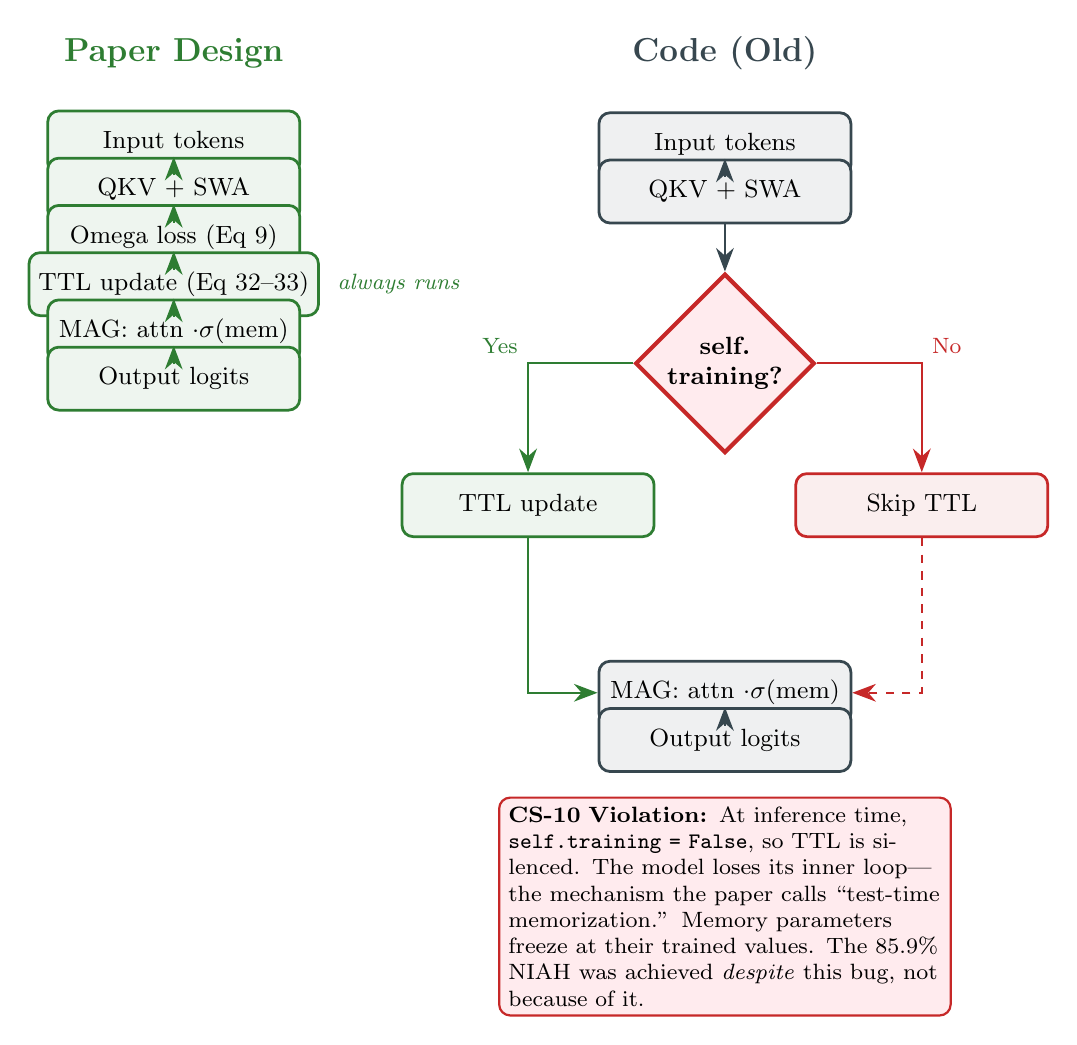
\begin{tikzpicture}[
  node distance=0.6cm and 1.2cm,
  every node/.style={font=\small},
  block/.style={
    rectangle, rounded corners=4pt, draw=#1, fill=#1!8,
    minimum width=3.2cm, minimum height=0.8cm, align=center,
    line width=1pt, font=\small
  },
  block/.default=codegray,
  arrow/.style={-{Stealth[length=3mm]}, thick, #1},
  arrow/.default=codegray,
]

% ══ Left: Paper's design (always-on TTL) ══
\node[font=\bfseries\large, eqgreen] (ptitle) at (-3.5, 0) {Paper Design};

\node[block=eqgreen, below=0.4cm of ptitle] (pinput) {Input tokens};
\node[block=eqgreen, below of=pinput] (pqkv) {QKV + SWA};
\node[block=eqgreen, below of=pqkv] (pomega) {Omega loss (Eq 9)};
\node[block=eqgreen, below of=pomega] (pttl) {TTL update (Eq 32--33)};
\node[block=eqgreen, below of=pttl] (pmag) {MAG: attn $\cdot\sigma$(mem)};
\node[block=eqgreen, below of=pmag] (pout) {Output logits};

\draw[arrow=eqgreen] (pinput) -- (pqkv);
\draw[arrow=eqgreen] (pqkv) -- (pomega);
\draw[arrow=eqgreen] (pomega) -- (pttl);
\draw[arrow=eqgreen] (pttl) -- (pmag);
\draw[arrow=eqgreen] (pmag) -- (pout);

\node[font=\footnotesize\itshape, eqgreen, right=0.1cm of pttl]
  {always runs};

% ══ Right: Code's design (training-gated TTL) ══
\node[font=\bfseries\large, codegray] (ctitle) at (3.5, 0) {Code (Old)};

\node[block, below=0.4cm of ctitle] (cinput) {Input tokens};
\node[block, below of=cinput] (cqkv) {QKV + SWA};

% The decision diamond
\node[diamond, draw=csred, fill=cslight, line width=1.5pt,
      below=0.6cm of cqkv, minimum width=2cm, minimum height=1.2cm,
      font=\small\bfseries, align=center, inner sep=1pt]
  (cdecision) {self.\\training?};

\node[block=eqgreen, below left=0.8cm and 0.3cm of cdecision] (cyes)
  {TTL update};
\node[block=csred, below right=0.8cm and 0.3cm of cdecision] (cno)
  {Skip TTL};

\node[block, below=2.6cm of cdecision] (cmag) {MAG: attn $\cdot\sigma$(mem)};
\node[block, below of=cmag] (cout) {Output logits};

\draw[arrow] (cinput) -- (cqkv);
\draw[arrow] (cqkv) -- (cdecision);
\draw[arrow=eqgreen] (cdecision) -| node[above left, font=\footnotesize] {Yes} (cyes);
\draw[arrow=csred] (cdecision) -| node[above right, font=\footnotesize] {No} (cno);
\draw[arrow=eqgreen] (cyes) |- (cmag);
\draw[arrow=csred, dashed] (cno) |- (cmag);
\draw[arrow] (cmag) -- (cout);

% ══ Annotation ══
\node[draw=csred, fill=cslight, rounded corners, thick,
      font=\footnotesize, align=left, text width=5.5cm,
      below=0.3cm of cout]
  (annotation) {%
    \textbf{CS-10 Violation:} At inference time,
    \texttt{self.training = False},
    so TTL is silenced. The model loses its inner loop---the
    mechanism the paper calls ``test-time memorization.''
    Memory parameters freeze at their trained values.
    The 85.9\% NIAH was achieved \emph{despite} this bug,
    not because of it.
  };

\end{tikzpicture}
\caption{\textbf{Behavioral Consequence of CS-10.} The paper's design (left)
runs TTL on every forward pass---training and inference alike. The code (right)
gates TTL behind \texttt{self.training}, disabling it during inference. This
single structural violation changes the model's behavior at test time.
Tests cannot catch this because tests run in training mode.}
\label{fig:behavioral}
\end{figure}

% ══════════════════════════════════════════════════════════════
\section{Figure 4: Equation Coverage vs.\ Structural Compliance}
% ══════════════════════════════════════════════════════════════

This figure shows the key asymmetry: perfect equation coverage coexists with
pervasive structural violation.

\begin{figure}[h!]
\centering
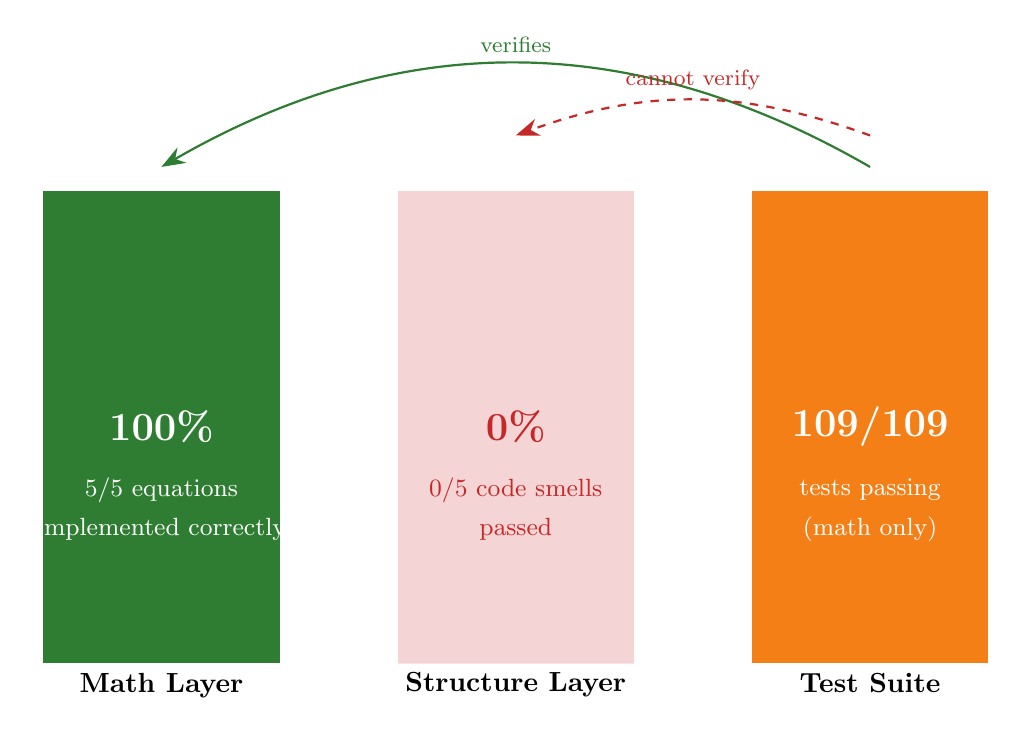
\begin{tikzpicture}[
  every node/.style={font=\small},
]

% ── Equation coverage (left bar) ──
\fill[eqgreen!20] (0,0) rectangle (3,6);
\fill[eqgreen] (0,0) rectangle (3,6);
\node[font=\Large\bfseries, white] at (1.5,3) {100\%};
\node[font=\small, white] at (1.5,2.2) {5/5 equations};
\node[font=\small, white] at (1.5,1.7) {implemented correctly};
\node[font=\bfseries, below] at (1.5,0) {Math Layer};

% ── Structure compliance (right bar) ──
\fill[csred!20] (4.5,0) rectangle (7.5,6);
\fill[csred] (4.5,0) rectangle (7.5,0);
\node[font=\Large\bfseries, csred] at (6,3) {0\%};
\node[font=\small, csred] at (6,2.2) {0/5 code smells};
\node[font=\small, csred] at (6,1.7) {passed};
\node[font=\bfseries, below] at (6,0) {Structure Layer};

% ── Test results ──
\fill[warnambr!20] (9,0) rectangle (12,6);
\fill[warnambr] (9,0) rectangle (12,6);
\node[font=\Large\bfseries, white] at (10.5,3) {109/109};
\node[font=\small, white] at (10.5,2.2) {tests passing};
\node[font=\small, white] at (10.5,1.7) {(math only)};
\node[font=\bfseries, below] at (10.5,0) {Test Suite};

% ── Arrows showing what tests cover ──
\draw[-{Stealth[length=3mm]}, thick, eqgreen]
  (10.5, 6.3) to[out=150, in=30] node[above, font=\footnotesize] {verifies} (1.5, 6.3);
\draw[-{Stealth[length=3mm]}, thick, csred, dashed]
  (10.5, 6.7) to[out=160, in=20]
  node[above, font=\footnotesize\color{csred}] {cannot verify} (6, 6.7);

\end{tikzpicture}
\caption{\textbf{The Coverage Gap.} The test suite verifies mathematical
correctness (green bar) but has no mechanism to verify structural compliance
(red bar). All 109 tests pass because they test equations, not ontology. The
graph fills this gap---code smell rules operate at the structural level that
tests cannot reach.}
\label{fig:coverage-gap}
\end{figure}

\clearpage

% ══════════════════════════════════════════════════════════════
\section{Figure 5: The Graph as Immune System}
% ══════════════════════════════════════════════════════════════

When code passes through the graph's code smell rules, structural violations
are detected before they propagate into the architecture.

\begin{figure}[h!]
\centering
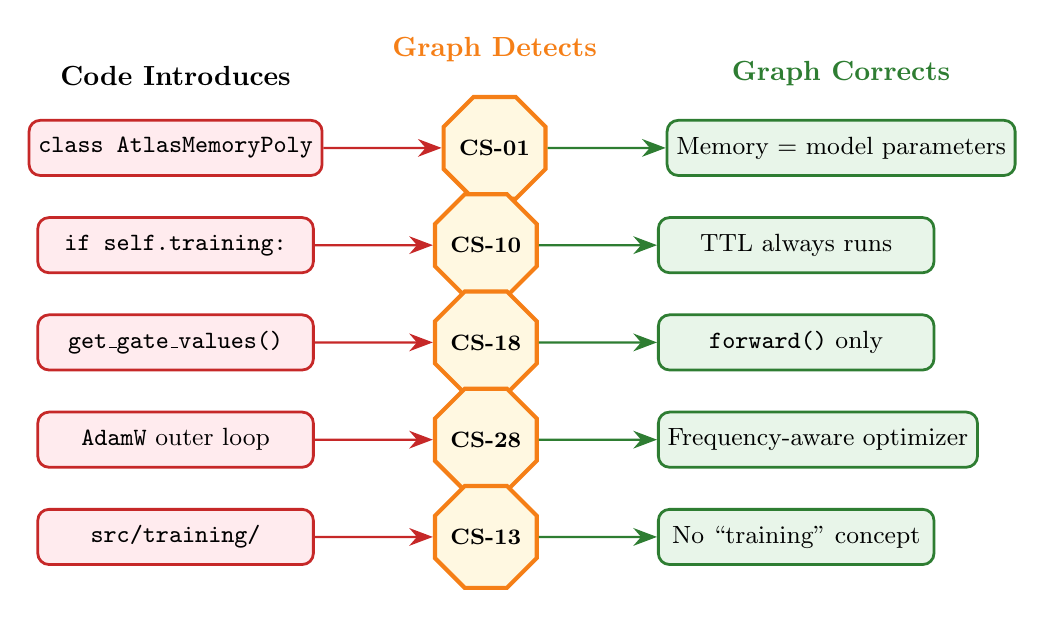
\begin{tikzpicture}[
  node distance=0.7cm and 1.5cm,
  every node/.style={font=\small},
  concept/.style={
    rectangle, rounded corners=4pt, draw=graphblue, fill=graphlight,
    minimum width=3.5cm, minimum height=0.7cm, align=center,
    line width=1pt
  },
  violation/.style={
    rectangle, rounded corners=4pt, draw=csred, fill=cslight,
    minimum width=3.5cm, minimum height=0.7cm, align=center,
    line width=1pt
  },
  detector/.style={
    regular polygon, regular polygon sides=8, draw=warnambr,
    fill=warnlight, minimum size=1.4cm, align=center,
    line width=1.5pt, font=\footnotesize\bfseries, inner sep=0pt
  },
  fix/.style={
    rectangle, rounded corners=4pt, draw=eqgreen, fill=eqlight,
    minimum width=3.5cm, minimum height=0.7cm, align=center,
    line width=1pt
  },
  arrow/.style={-{Stealth[length=3mm]}, thick},
]

% Row 1: Code introduces violation
\node[violation] (v1) at (0, 0) {\texttt{class AtlasMemoryPoly}};
\node[detector, right=1.5cm of v1] (d1) {CS-01};
\node[fix, right=1.5cm of d1] (f1) {Memory = model parameters};
\draw[arrow, csred] (v1) -- (d1);
\draw[arrow, eqgreen] (d1) -- (f1);

\node[violation, below=0.5cm of v1] (v2) {\texttt{if self.training:}};
\node[detector, right=1.5cm of v2] (d2) {CS-10};
\node[fix, right=1.5cm of d2] (f2) {TTL always runs};
\draw[arrow, csred] (v2) -- (d2);
\draw[arrow, eqgreen] (d2) -- (f2);

\node[violation, below=0.5cm of v2] (v3) {\texttt{get\_gate\_values()}};
\node[detector, right=1.5cm of v3] (d3) {CS-18};
\node[fix, right=1.5cm of d3] (f3) {\texttt{forward()} only};
\draw[arrow, csred] (v3) -- (d3);
\draw[arrow, eqgreen] (d3) -- (f3);

\node[violation, below=0.5cm of v3] (v4) {\texttt{AdamW} outer loop};
\node[detector, right=1.5cm of v4] (d4) {CS-28};
\node[fix, right=1.5cm of d4] (f4) {Frequency-aware optimizer};
\draw[arrow, csred] (v4) -- (d4);
\draw[arrow, eqgreen] (d4) -- (f4);

\node[violation, below=0.5cm of v4] (v5) {\texttt{src/training/}};
\node[detector, right=1.5cm of v5] (d5) {CS-13};
\node[fix, right=1.5cm of d5] (f5) {No ``training'' concept};
\draw[arrow, csred] (v5) -- (d5);
\draw[arrow, eqgreen] (d5) -- (f5);

% Column labels
\node[font=\bfseries, above=0.3cm of v1] {Code Introduces};
\node[font=\bfseries\color{warnambr}, above=0.3cm of d1] {Graph Detects};
\node[font=\bfseries\color{eqgreen}, above=0.3cm of f1] {Graph Corrects};

\end{tikzpicture}
\caption{\textbf{The Graph as Immune System.} Each code smell rule (octagon)
detects a specific class of structural violation. Violations enter from the
left (red); the graph rejects them and prescribes corrections (green, right).
Without the graph, all five violations passed through 109 tests undetected.}
\label{fig:immune-system}
\end{figure}


% ══════════════════════════════════════════════════════════════
\section{Detailed Violation Catalog}
% ══════════════════════════════════════════════════════════════

\begin{table}[h!]
\centering
\small
\begin{tabular}{@{}llp{4.2cm}p{4.2cm}l@{}}
\toprule
\textbf{Rule} & \textbf{File} & \textbf{Violation} & \textbf{Paper Says} & \textbf{Severity} \\
\midrule
CS-01 & atlas\_memory.py &
  Memory is a separate \texttt{nn.Module} with own \texttt{forward()} &
  Memory IS the parameters of the MLP; no separate module boundary &
  High \\
\addlinespace
CS-10 & blocks.py:245 &
  \texttt{if self.training:} gates TTL &
  No mode distinction; TTL runs on every forward pass (``test-time'' learning) &
  \textbf{Critical} \\
\addlinespace
CS-13 & src/training/ &
  Directory named ``training''; concepts use training terminology &
  Context processing is continuous; ``training'' implies a phase that ends &
  Low \\
\addlinespace
CS-18 & skeleton.py &
  5 extra methods: \texttt{forward\_memory\_only}, \texttt{get\_gate\_values}, etc. &
  Forward pass IS the only external API &
  Medium \\
\addlinespace
CS-28 & train.py &
  AdamW used for outer loop optimization &
  Outer loop must be frequency-aware; Muon/M3 family &
  Medium \\
\bottomrule
\end{tabular}
\caption{Complete catalog of structural violations detected by graph audit.
CS-10 is the only violation that changes model \emph{behavior}; the others
affect code organization and conceptual clarity.}
\label{tab:violations}
\end{table}

% ══════════════════════════════════════════════════════════════
\section{Invented Concepts}
% ══════════════════════════════════════════════════════════════

Beyond code smell violations, the implementation introduces concepts with
\textbf{no paper origin}:

\begin{table}[h!]
\centering
\small
\begin{tabular}{@{}lp{5cm}p{5cm}@{}}
\toprule
\textbf{Invented Concept} & \textbf{What It Does} & \textbf{Why It's Wrong} \\
\midrule
\texttt{PersistentMemory} &
  Precomputed $M_\text{persistent}$ from ``learned persistent keys'' &
  Paper has no persistent memory for Omega Rule. Correct init is $M_0 = 0$. \\
\addlinespace
\texttt{output\_scale} &
  Learnable scalar (init 0.15) to match attention magnitude &
  Paper's MAG uses $\sigma(\text{mem})$ which already bounds to $[0,1]$.
  Extra scale distorts the gating signal. \\
\addlinespace
\texttt{TTLUpdater} class &
  Stateful wrapper with reset modes and step counting &
  The inner loop is a mathematical operation (Eqs 32--33), not a
  stateful object with lifecycle methods. \\
\addlinespace
\texttt{poly\_norm} &
  LayerNorm on polynomial features before MLP &
  Paper specifies $\varphi(x) = [x, x_i x_j]$ directly into MLP.
  Normalization changes the feature distribution. \\
\bottomrule
\end{tabular}
\caption{Concepts invented during implementation that have no basis in the paper.
Each represents architectural drift---a small decision that compounds over
4 months of development.}
\label{tab:invented}
\end{table}

% ══════════════════════════════════════════════════════════════
\section{What Tests Cannot Catch}
% ══════════════════════════════════════════════════════════════

The fundamental insight of this audit:

\begin{quote}
\emph{Tests verify that code computes the right answer.\\
The graph verifies that code asks the right question.}
\end{quote}

\noindent All 109 tests verify mathematical properties:
\begin{itemize}[nosep]
  \item Newton-Schulz produces near-orthogonal matrices ($\|XX^T - I\|_F < \epsilon$)
  \item Polynomial features have correct output dimension ($d_k + \binom{d_k+1}{2}$)
  \item Omega loss decreases with more context tokens
  \item TTL step reduces memory prediction error
  \item MAG gating is bounded in $[0,1]$
\end{itemize}

\noindent None of the 109 tests verify structural properties:
\begin{itemize}[nosep]
  \item Does TTL run during inference? (No---\texttt{self.training} blocks it)
  \item Is memory a separate module? (Yes---violates CS-01)
  \item Does the model expose multiple APIs? (Yes---5 extra methods beyond \texttt{forward})
  \item Are invented concepts present? (Yes---persistent memory, output scale)
\end{itemize}

\noindent The graph's code smell rules are the \textbf{structural type system}
that tests cannot replace.

% ══════════════════════════════════════════════════════════════
\section{Conclusion}
% ══════════════════════════════════════════════════════════════

The Atlas-MAG implementation demonstrates that \textbf{mathematical correctness
is necessary but not sufficient}. A codebase can implement every equation
faithfully, pass every test, and still violate the paper's design at the
structural level.

The NL graph methodology addresses this gap through:
\begin{enumerate}[nosep]
  \item \textbf{Equation nodes} that ensure mathematical traceability
  \item \textbf{Code smell rules} that enforce structural compliance
  \item \textbf{IS/IS NOT axiom containers} that reject foreign concepts
  \item \textbf{Pseudocode generation} from graph nodes (not from human interpretation)
\end{enumerate}

The old Atlas-MAG code is now archived as a historical artifact---a controlled
example of what paper-to-code looks like \emph{without} the graph. The new
pseudocode (5 tiers, 38 equations traced) shows what the graph \emph{produces}.
The contrast between the two is the methodology's evidence.

\vfill
\noindent\rule{\textwidth}{0.4pt}\\
{\footnotesize
  \textbf{Graph source:} \texttt{HADES\_DATABASE=NL}, collections:
  \texttt{atlas\_equations} (60), \texttt{atlas\_axioms} (2),
  \texttt{nl\_code\_smells} (36)\\
  \textbf{Old code:} \texttt{github.com/toddwbucy/Atlas-MAG\_OmegaRule} (archived)\\
  \textbf{New pseudocode:} \texttt{github.com/toddwbucy/Atlas} (5 tiers)\\
  \textbf{Generated:} \today
}

\end{document}
